\section{Results}
\label{sec:results}
The combined method reduces the time for the final collection, but the contribution depends on the physical structure and on how the requests are processed. We first report the complete comparison, then the individual families and learned components.

\subsection{Complete time for the final 93 requests}
The final application takes a median of 41.137 seconds, compared with 45.091 seconds for the preceding application. The ratio is 0.912, which corresponds to 8.8\% less time. Table~\ref{tab:final-times} gives all three measured procedures, and Figure~\ref{fig:final-times} shows each repetition. All 837 application results, from 93 requests, three methods, and three repetitions, pass the 13,401 exact coefficient comparisons. No internal native attempt fails in this final serial comparison.

\begin{table}[!htbp]\centering
\caption{Complete-collection elapsed time for 93 matched requests. The ranges contain the three observed times; they are not confidence intervals. All methods process the collection in one call.}
\label{tab:final-times}
\begin{tabular}{@{}lrr@{}}\toprule
Application & Median (s) & Observed range (s)\\\midrule
Preceding & 45.091 & 44.783--45.817\\
Intermediate & 42.932 & 40.351--44.589\\
Final & 41.137 & 40.723--41.227\\\bottomrule
\end{tabular}
\end{table}

\begin{figure}[!htbp]\centering
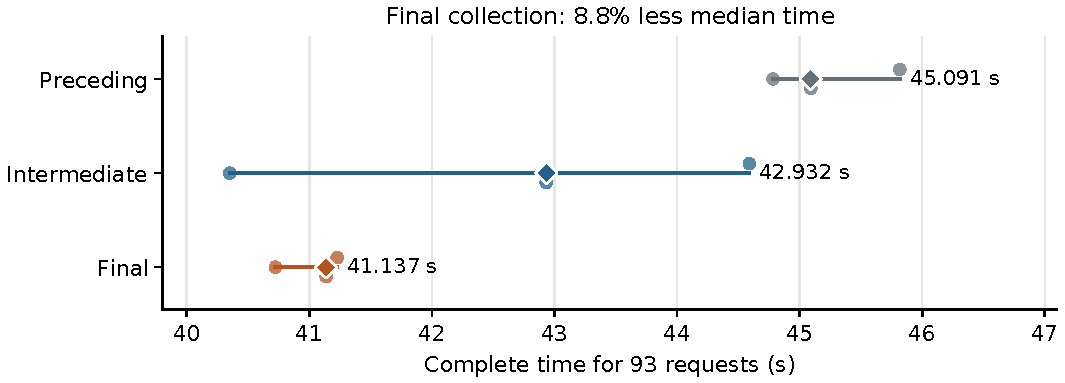
\includegraphics[width=.96\linewidth]{paper_figures/rewrite_total.pdf}
\caption{The final method reduces complete-collection time in each recorded repetition. Points are the three observations for each method; diamonds are their medians. The elapsed-time axis is restricted to the observed range so that the comparison remains readable. All points include shared setup and recovery costs.}
\label{fig:final-times}
\end{figure}
The intermediate-to-final difference is smaller than the preceding-to-final difference and varies with the execution conditions. The monitor correction removes a reproduced interruption mechanism, but these timings alone do not assign all of their difference to that correction. The scientific result is the measured total change of the combined procedure.

\subsection{Which integral structures become faster}
Table~\ref{tab:group-times} shows the native groups within the final shared-call experiment. Planar and nonplanar boxes become faster, while the sunrise group becomes slower and the three-loop vacuum group changes little. Thus an aggregate improvement does not imply an improvement for every family. The component times also show that the remaining native algebra dominates this particular collection.

\begin{table}[!htbp]\centering\small
\caption{Native component times inside the final shared-call comparison. Each entry is a sum of per-request medians for five requests. Ratios divide final time by preceding time; shared overhead is excluded from these component sums.}
\label{tab:group-times}
\begin{tabular}{@{}lrrr@{}}\toprule
Structure & Preceding (s) & Final (s) & Ratio\\\midrule
Planar box & 8.948 & 7.191 & 0.804\\
Nonplanar box & 14.517 & 11.137 & 0.767\\
Massive sunrise & 7.509 & 8.407 & 1.120\\
Three-loop vacuum & 12.971 & 12.988 & 1.001\\\bottomrule
\end{tabular}
\end{table}
The separate fresh-call experiment asks a different question: how much time each new request needs when it starts its own application. Across its 40 requests, summed median time falls from 57.766 to 50.848 seconds, a ratio of 0.880. The paired request-resampling interval is $[0.744,0.992]$. The 20 native requests alone give 0.887 with interval $[0.743,1.010]$, which includes equal time. These results refer to the direct triangle and native-setting changes before the final monitor correction.

Figure~\ref{fig:scope-times} shows the fresh-call change by physical structure and the triangle-product points at each loop order. The triangle group gives a ratio of 0.816, but the seven-loop product gives 1.077 and is slower. Higher-loop products test the factorization identity under the specified powers and invariants. They supply no timing result for a general connected scattering graph at the same loop order.
\begin{figure}[!htbp]\centering
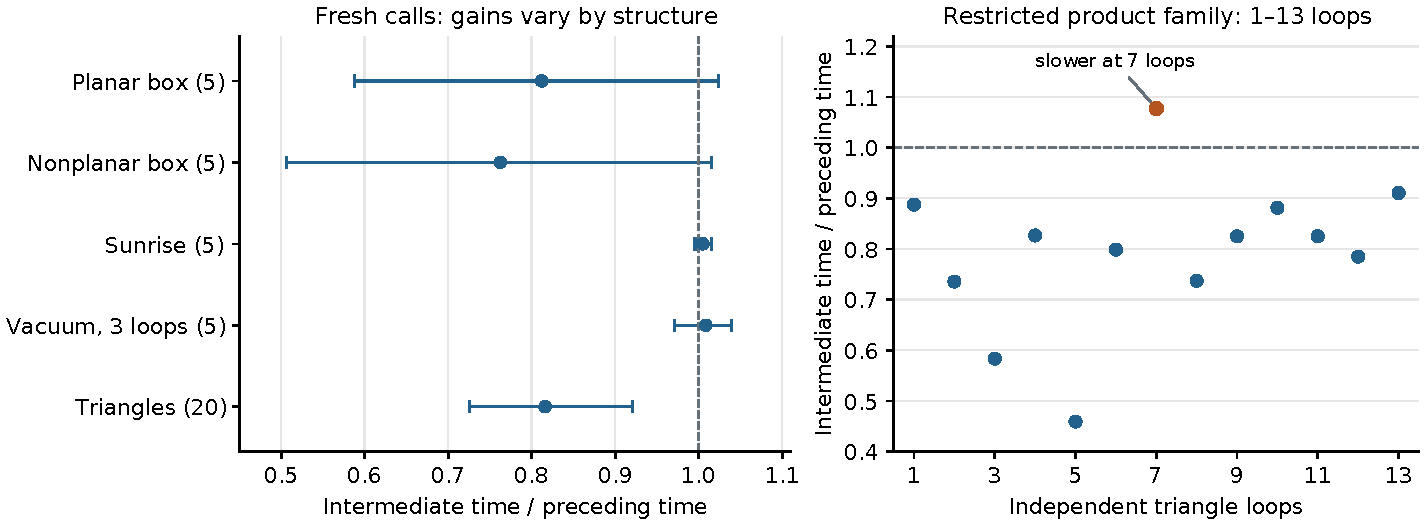
\includegraphics[width=\linewidth]{paper_figures/rewrite_scope.pdf}
\caption{The fresh-call gain depends on the input. Left: ratio of summed median times for each group; each entry uses the same requests in both methods, with request counts in parentheses. Horizontal bars are central 95\% paired-request bootstrap intervals. Right: triangle-product ratios at loop orders one through thirteen. There are eight requests at one loop and one at each higher loop order; the right panel therefore shows point estimates without intervals. Values below the dashed line mean less time. These plots show the intermediate method against the preceding method, and use a different timing protocol from Figure~\ref{fig:final-times}.}
\label{fig:scope-times}
\end{figure}

\subsection{How much of the gain comes from machine learning}
\label{sec:ml-results}
Earlier controlled tests resolve small seed-selection and equation-selection gains on their stated workloads (Table~\ref{tab:ml-results}). These results motivated the learned interventions. The row model took more time, and a later compiled row policy had an interval that included equal time. We therefore retain Kira's native row choices.

\begin{table}[!htbp]\centering\small
\caption{Separate learned-component comparisons from this study. Ratios below one mean less time. The workloads and controls differ, so the ratios cannot be combined into one speed factor. Intervals retain the original study's resampling units, specified below.}
\label{tab:ml-results}
\begin{tabularx}{\linewidth}{@{}YYrr@{}}\toprule
Learned component & Control and workload & Ratio & Interval\\\midrule
Earlier seed model & Fixed seed region; 32 box batches & 0.963 & $[0.937,0.984]$\\
Earlier equation model & Native filter; 24 new-index batches & 0.933 & $[0.928,0.940]$\\
Original row model & Native row choices; 84 trials & 1.305 & ---\\
Compiled row-cost policy & Native choices; geometric-mean estimator & 0.982 & $[0.959,1.003]$\\
Inherited learned choices with reconstruction & Fixed choices, same arithmetic; 22 native requests & 0.983 & $[0.951,1.003]$\\\bottomrule
\end{tabularx}
\end{table}
The seed and reconstruction-era intervals resample requests; the equation interval resamples paired repetitions on fixed requests. The equation timer includes its coefficient checks and excludes initial imports, whereas the final collection has the timing boundary in Section~\ref{sec:design}. The compiled-row interval retains its original grouped estimator. These differences are another reason to keep the comparisons separate.

The last row tests the inherited learned choices after the arithmetic changes. Its fixed and learned times are 42.175 and 41.448 seconds, respectively, but the interval includes equal time. It therefore does not establish a reliable additional aggregate gain from those learned choices on that sample. Both procedures complete all requests without an unsuccessful internal attempt.

The latest arithmetic selector also fails its validation condition. Its best fitted choice has 46.495 seconds of validation cost, compared with 46.438 seconds for the structure-dependent fixed settings. The required three-percent gain is absent, so the added selector is disabled. Similarly, the nonplanar equation filter takes 16.807 seconds against 9.824 seconds without the filter. It skips 17,808 of 53,430 candidate equation constructions, but all ten filtered attempts fail to reach the prescribed master basis and need recovery. This test demonstrates why equation counts alone cannot establish a time gain.

\begin{figure}[!htbp]\centering
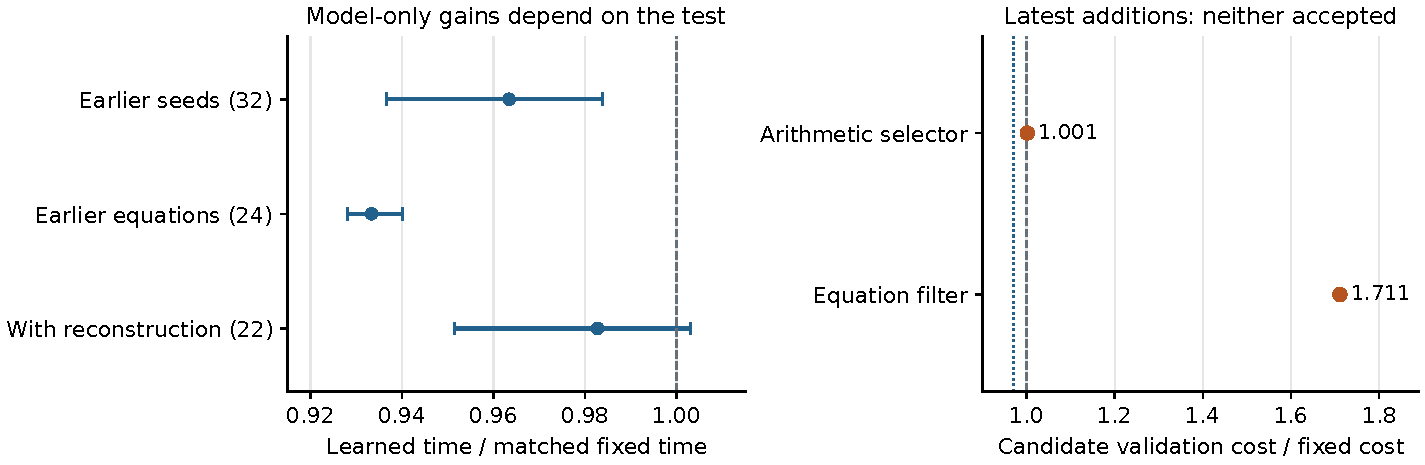
\includegraphics[width=\linewidth]{paper_figures/rewrite_ml.pdf}
\caption{Learned improvements are specific to a tested setting. Left: three model-only time ratios with their recorded resampling intervals and request counts. The seed and reconstruction intervals resample requests; the equation interval resamples paired repetitions. The reconstruction-era interval includes equal time. Right: latest validation costs, normalized to the matched fixed control. The additional arithmetic selector and equation filter remain disabled. The dashed line marks equal cost, and the dotted line marks the arithmetic selector's 0.97 acceptance threshold.}
\label{fig:ml-controls}
\end{figure}

\subsection{Earlier combined gains and unsuccessful comparisons}
The earlier 75-request experiment measures the effect of adding validated coefficient reconstruction to an application that already has direct vacuum formulas. Summed median time changes from 79.624 to 49.852 seconds, or 37.4\% less time. The directly matched comparison across both the vacuum and reconstruction changes gives 81.827 to 49.852 seconds, or 39.1\% less time. The latter is a cumulative result on one workload. Its control is an earlier application, not unmodified Kira, and its percentage is separate from the final 93-request result.

An initial parallel version of the final comparison stopped before all three repetitions finished. Of 651 recorded request results, 650 passed and one preceding-method vacuum result failed the prescribed-basis check. After an interrupted attempt, recovery returned 20 masters while the reference used 16. No conversion between those bases was performed, so the test did not establish whether the returned expressions were equivalent. We preserve this failed comparison and exclude its incomplete repetition from the timing estimator. The serial experiment of Table~\ref{tab:final-times} is complete; it does not erase the earlier failure. The notes retain the full interrupted experiment, older timing protocols, and model-training results.
\FloatBarrier
